\documentclass[10pt,a4paper]{article}
\usepackage[margin=.8in]{geometry}\usepackage[T1]{fontenc}
\usepackage{lmodern,microtype,booktabs,graphicx,xcolor,hyperref}
\hypersetup{hidelinks}\setlength{\parindent}{0pt}\setlength{\parskip}{6pt}
\title{IDM-Viz: Released-Label Recalibration on ELEC2}
\author{Ahmed Bilal (23I-2581) \and Umar Behram (23I-2604)}\date{16 November 2026}
\begin{document}\maketitle
\begin{abstract}
We tested whether updating only the correctness calibrator with monitoring labels released strictly before each forecast improves current-batch accuracy estimates on the ELEC2 stream. Recalibration reduced average signed bias toward zero but did not reduce equal-batch MAE at any tested delay; interval coverage also did not consistently improve. This is one outcome-informed stream analysis, not a general recalibration result.
\end{abstract}
\section{Protocol}
The classifier, features, training scaler and predictions are unchanged from the ELEC2 base run. A frozen isotonic calibrator is compared with a new isotonic calibrator refit on the original calibration examples plus all monitoring confidence/correctness pairs whose labels were released strictly before the current batch forecast. Same-clock labels are added only after that forecast is persisted, including at zero delay. Delays are 0, 5 and 20 batches. The classifier is not retrained. All 55 monitoring batches, including the final partial batch, are included.
\section{Results}
\begin{table}[ht]\centering\small
\caption{Equal-batch estimation errors and exact plug-in interval coverage. No inferential intervals are reported because this is one serial stream.}
\resizebox{\linewidth}{!}{%
\begin{tabular}{rrrrrrr}\toprule Delay & Frozen MAE & Updated MAE & Frozen bias & Updated bias & Frozen coverage & Updated coverage \\\midrule
0 & 0.059 & 0.063 & -0.011 & -0.000 & 23/55 & 18/55 \\
5 & 0.059 & 0.064 & -0.011 & -0.002 & 23/55 & 21/55 \\
20 & 0.059 & 0.059 & -0.011 & -0.002 & 23/55 & 24/55 \\
\bottomrule\end{tabular}}
\end{table}
Frozen equal-batch MAE was 0.0586 for all delay settings. Recalibrated MAE was 0.0628, 0.0637 and 0.0591 at delays 0, 5 and 20, respectively. Recalibration moved signed bias from -0.0106 toward zero (to -0.0005, -0.0023 and -0.0018) but did not yield lower MAE. Empirical interval coverage was 23/55 for the frozen estimator and 18/55, 21/55 and 24/55 after recalibration. Correctness Brier scores were similar and mixed across delays.
\begin{figure}[ht]\centering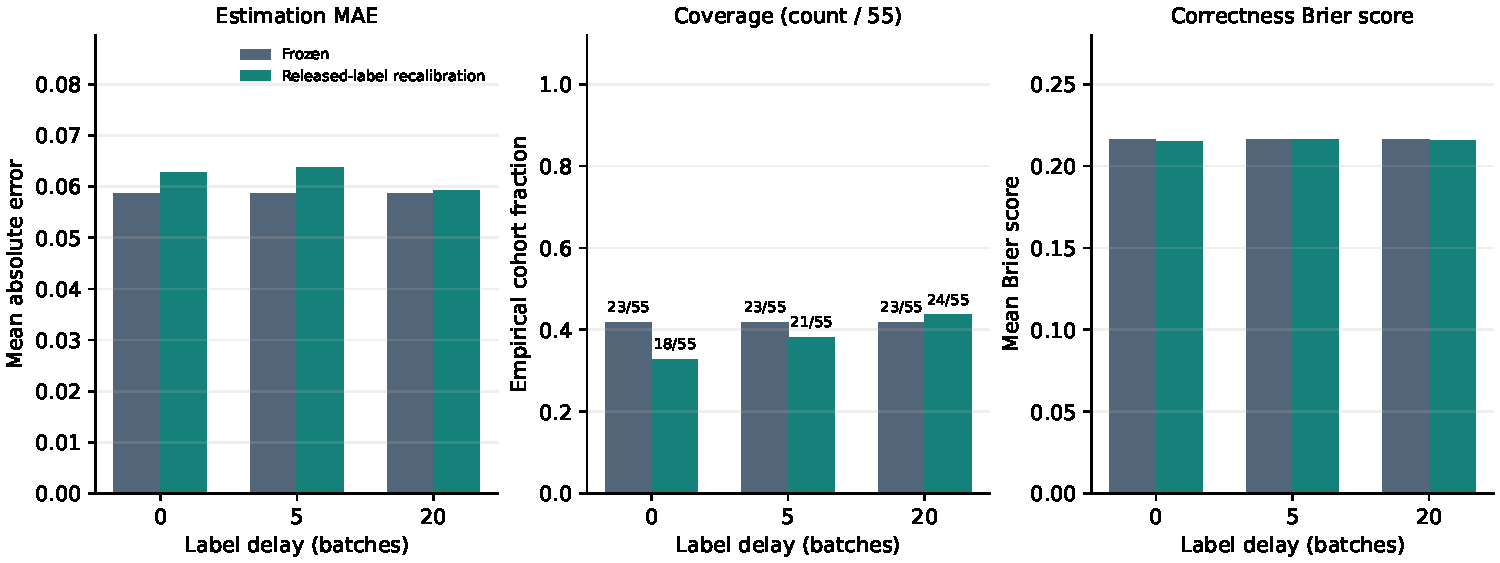
\includegraphics[width=.98\linewidth]{recalibration_tradeoff.pdf}
\caption{Frozen versus released-label recalibration by delay. Coverage bars show cohort counts out of 55.}
\end{figure}
\section{Interpretation and limits}
The evidence does not support claiming that simple cumulative isotonic recalibration fixes this stream's estimator. Reduced aggregate bias can coexist with increased MAE and worse interval coverage. Delay comparisons have unequal available label budgets by design. Batches are serial and dependent, so the 55 cohorts are not independent replicates. The experiment uses one fixed stream, one model and an outcome-informed extension; calibration, reference and stream uncertainty are not certified. Recalibration does not establish improved classification accuracy or future-harm prediction.
\section{Reproduction}
\begin{verbatim}
python scripts/run_elec2_delayed_recalibration.py `
  --run results/phase3/elec2_NEW `
  --out results/phase3/recal_NEW
python scripts/evaluate_elec2_delayed_recalibration.py `
  --run results/phase3/elec2_NEW `
  --recalibration results/phase3/recal_NEW
python scripts/report_elec2_delayed_recalibration.py
\end{verbatim}
\end{document}
